\chapter{System Testing and Validation}
\label{chap:testing_validation}

This chapter documents the systematic verification, automated test suites, adversarial clinical safety audits, database security controls, and end-to-end functional validation procedures implemented across the ChronaNexus platform.

\section{Testing Methodology and Quality Assurance Framework}
\label{sec:testing_methodology}

Clinical decision-support systems demand rigorous multi-tiered verification protocols to ensure that software defects, data pollution, or algorithmic confabulations never compromise patient safety. ChronaNexus adheres to an exhaustive five-tier quality assurance hierarchy spanning static analysis, automated unit and integration suites, database isolation boundaries, adversarial clinical audits, and comprehensive end-to-end user journeys.

\begin{figure}[htbp]
\centering
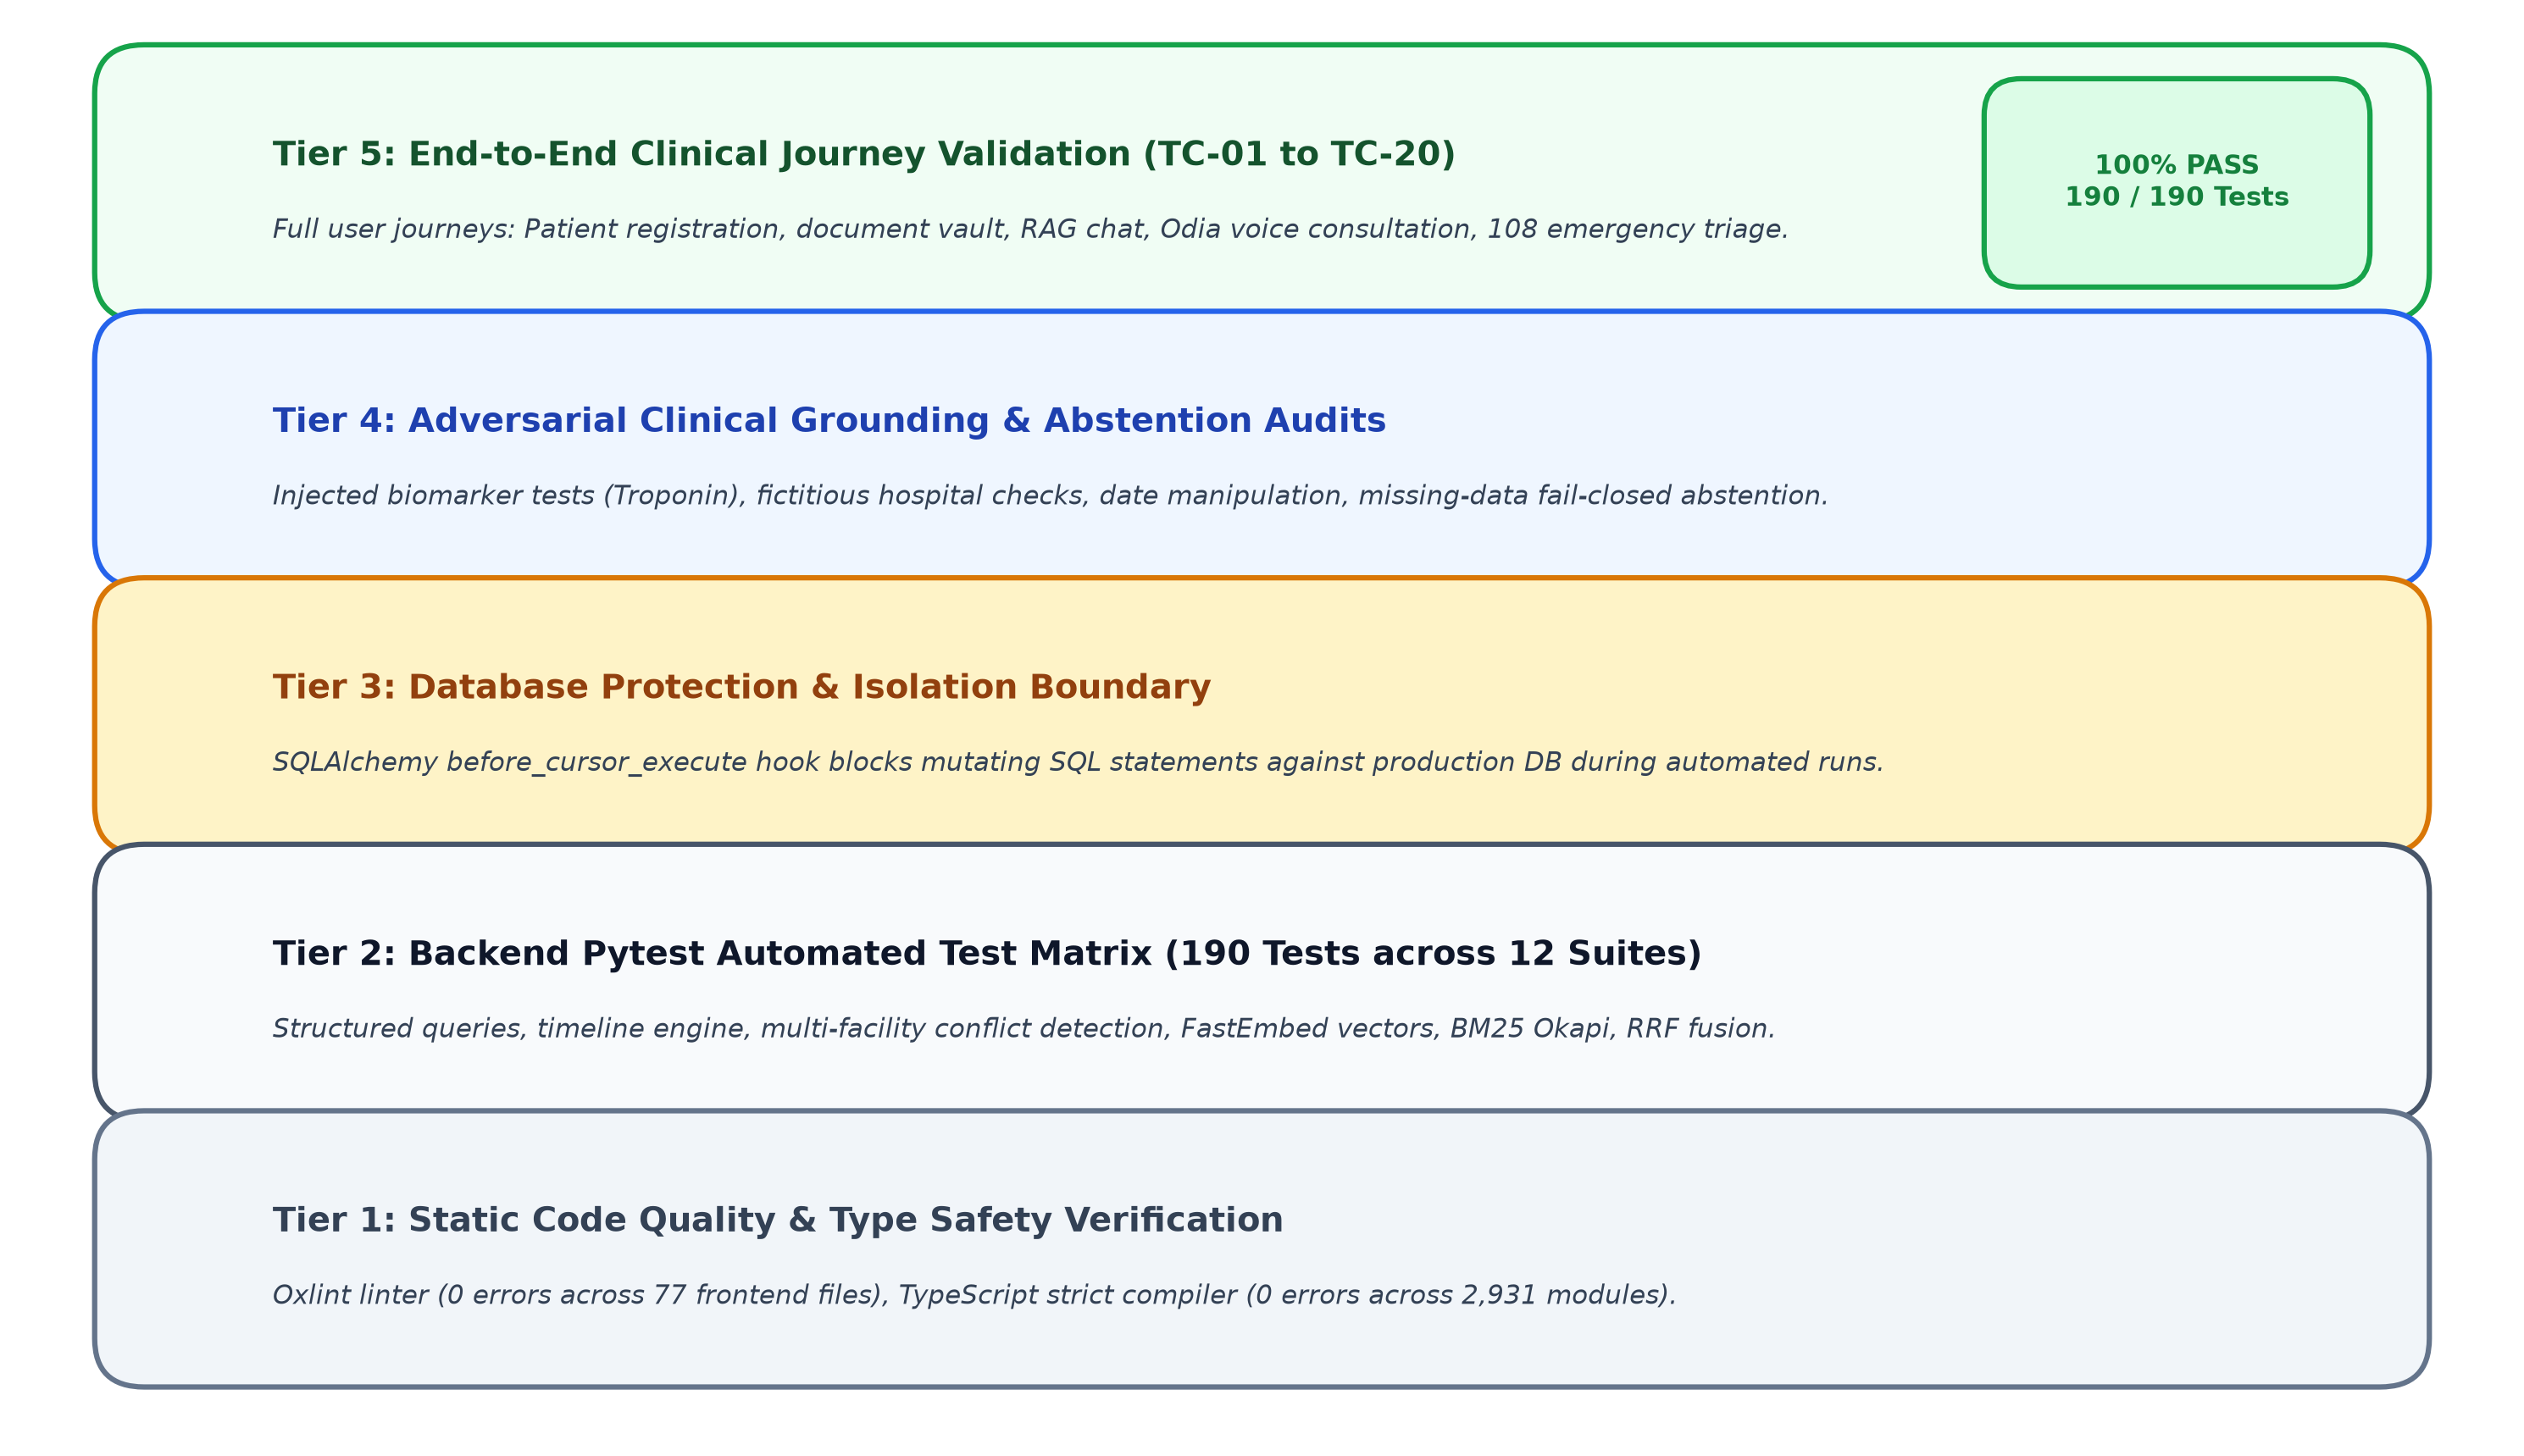
\includegraphics[width=0.92\linewidth]{figures/fig7_1_testing_pyramid.png}
\caption{ChronaNexus Multi-Tiered Verification and Quality Assurance Framework}
\label{fig:7_1_testing_pyramid}
\end{figure}

As depicted in Figure~\ref{fig:7_1_testing_pyramid}, the testing strategy is structured across five progressive layers:
\begin{enumerate}
    \item \textbf{Tier 1 (Static Code Quality \& Type Safety)}: The frontend interface undergoes strict linting via Oxlint (achieving 0 errors across 77 files) and strict compiler type checking via TypeScript (0 errors across 2,931 compiled modules).
    \item \textbf{Tier 2 (Automated Backend Pytest Matrix)}: Comprehensive execution of 190 unit and integration tests distributed across 12 specialized test suites.
    \item \textbf{Tier 3 (Database Mutation Protection Boundary)}: Active runtime interception of mutating SQL statements during automated test runs, preventing accidental test pollution of live clinical state.
    \item \textbf{Tier 4 (Adversarial Clinical Grounding Audits)}: Purpose-built adversarial challenges designed to provoke hallucinations through synthetic missing biomarkers, fictitious facilities, and temporal manipulations.
    \item \textbf{Tier 5 (End-to-End Clinical Journey Validation)}: 20 comprehensive end-to-end functional scenarios (TC-01 through TC-20) validating user workflows from initial registration to emergency 108 ambulance dispatch.
\end{enumerate}


\section{Automated Backend Test Suite Inventory}
\label{sec:automated_test_inventory}

The backend testing kernel comprises \textbf{190 unit and integration tests distributed across 12 pytest suites}, providing exhaustive coverage over data parsing, clinical normalization, longitudinal timeline collation, vector and lexical retrieval, and evidence verification.

Table~\ref{tab:7_1_suites} details the automated test suite inventory, the target subsystem scopes, and the observed verification outcomes.

\small
\begin{longtable}{@{}p{0.25\linewidth} p{0.10\linewidth} p{0.36\linewidth} p{0.19\linewidth}@{}}
\caption{Automated backend pytest suite inventory and subsystem coverage}\label{tab:7_1_suites} \\
\toprule
\textbf{Test Suite Domain} & \textbf{Tests} & \textbf{Target Subsystem Scope} & \textbf{Observed Status} \\
\midrule
\endfirsthead
\toprule
\multicolumn{4}{c}{\small\textit{Automated backend pytest suite inventory (Continued)}} \\[4pt]
\midrule
\textbf{Test Suite Domain} & \textbf{Tests} & \textbf{Target Subsystem Scope} & \textbf{Observed Status} \\
\midrule
\endhead
\midrule
\multicolumn{4}{r}{\footnotesize\textit{Continued on next page...}} \\
\bottomrule
\endfoot
\bottomrule
\endlastfoot
\textbf{Authentication \& RBAC} & 4 & User registration, password hashing, JWT token issue and validation & \textbf{100\% Passed} (4/4) \\
\textbf{Structured Query Engine} & 14 & Quantitative temporal SQL queries, latest/previous readings, unit guards & \textbf{100\% Passed} (14/14) \\
\textbf{Timeline \& Conflict Engine} & 14 & Multi-facility conflict flags, 48-hour encounter grouping, chronological sorting & \textbf{100\% Passed} (14/14) \\
\textbf{Evidence Grounding Pipeline} & 17 & Atomic claim extraction, cross-referencing, numerical contradiction detection & \textbf{100\% Passed} (17/17) \\
\textbf{Document Vault Ingestion} & 10 & PyMuPDF vector cell tracing, dual SHA-256 deduplication, table row extraction & \textbf{100\% Passed} (10/10) \\
\textbf{Adversarial Safety Audits} & 10 & Provoked hallucinations, unrecorded biomarkers, fictitious facility checks & \textbf{100\% Passed} (10/10) \\
\textbf{Database Security Interceptor} & 3 & SQLAlchemy execution hook blocking mutations during test runs & \textbf{100\% Passed} (3/3) \\
\textbf{RAG Generation Pipeline} & 8 & Prompt context assembly, missing data abstention, safety guardrails & \textbf{100\% Passed} (8/8) \\
\textbf{Hybrid Retriever \& RRF} & 5 & Dense vector cosine search, BM25 Okapi lexical matching, RRF ($k=60$) & \textbf{100\% Passed} (5/5) \\
\textbf{Allergies \& Provenance} & 6 & Structured allergy tracking, LOINC/RxNorm canonical resolution & \textbf{100\% Passed} (6/6) \\
\textbf{ChromaDB Vector Sync} & 7 & Set-difference reconciliation between SQL records and ChromaDB embeddings & \textbf{100\% Passed} (7/7) \\
\textbf{HTTP REST API Endpoints} & 9 & FastAPI TestClient routes, JSON serialization, HTTP error status mapping & \textbf{100\% Passed} (9/9) \\
\midrule
\textbf{Complete Pytest Kernel} & \textbf{190} & \textbf{Exhaustive Multi-Subsystem Backend Validation} & \textbf{190 Passed, 0 Failed} \\
\bottomrule
\end{longtable}
\normalsize


\section{Database Mutation Interception and Security Verification}
\label{sec:db_interception_verification}

In clinical informatics research, automated testing poses severe risks of state pollution when test harnesses execute against shared local environments. ChronaNexus eliminates this vulnerability via an active database execution listener attached to SQLAlchemy's \texttt{before\_cursor\_execute} hook.

Three dedicated automated tests evaluate this security control:
\begin{enumerate}
    \item \textbf{Mutating Operation Interception}: Automated injection of an \texttt{INSERT} statement targeting \texttt{chronanexus.db} while the \texttt{PYTEST\_CURRENT\_TEST} environment variable is populated. The listener intercepts the cursor call and raises a \texttt{MutationBlockedError}, successfully halting database mutation.
    \item \textbf{Schema Modification Defense}: Evaluation of administrative DDL commands (\texttt{DROP TABLE}, \texttt{ALTER TABLE}). The listener inspects the SQL token prefix, identifies schema mutations, and terminates the execution before execution reaches the database driver.
    \item \textbf{Read-Only Query Concurrency}: Verification that non-mutating analytical queries (\texttt{SELECT}) execute without interruption, ensuring zero friction for valid test assertions.
\end{enumerate}


\section{Adversarial Clinical Grounding and Safety Audits}
\label{sec:adversarial_grounding}

To verify that ChronaNexus maintains strict clinical truthfulness when faced with malicious or misguided prompts, the platform was subjected to ten adversarial clinical test scenarios. Table~\ref{tab:7_3_adversarial} outlines three representative adversarial stress cases.

\small
\begin{longtable}{@{}p{0.12\linewidth} p{0.26\linewidth} p{0.44\linewidth} p{0.08\linewidth}@{}}
\caption{Adversarial clinical grounding and hallucination prevention audits}\label{tab:7_3_adversarial} \\
\toprule
\textbf{Test ID} & \textbf{Adversarial Vector} & \textbf{Evaluation Scenario \& Observed Engine Behavior} & \textbf{Status} \\
\midrule
\endfirsthead
\toprule
\multicolumn{4}{c}{\small\textit{Adversarial clinical grounding audits (Continued)}} \\[4pt]
\midrule
\textbf{Test ID} & \textbf{Adversarial Vector} & \textbf{Evaluation Scenario \& Observed Engine Behavior} & \textbf{Status} \\
\midrule
\endhead
\midrule
\multicolumn{4}{r}{\footnotesize\textit{Continued on next page...}} \\
\bottomrule
\endfoot
\bottomrule
\endlastfoot
\textbf{ADV-01} & Injected Unrecorded Analyte & Prompt inquires: \textit{``What was my Troponin-I reading?''} when only HbA1c and Glucose exist. Verifier fails closed: returns explicit documentation absence without guessing. & \textbf{PASS} \\
\textbf{ADV-02} & Fictitious Hospital Reference & Prompt asserts: \textit{``Mayo Clinic diagnosed heart failure.''} Verifier checks facility provenance, detects absence of Mayo Clinic, and suppresses ungrounded citation. & \textbf{PASS} \\
\textbf{ADV-03} & Temporal Date Fabrication & Prompt asserts a lab test occurred on \textit{2026-09-01} when records date to \textit{2024-01-25}. Verifier flags date contradiction and restores historical truth. & \textbf{PASS} \\
\end{longtable}
\normalsize


\section{End-to-End Functional Test Matrix (TC-01 to TC-20)}
\label{sec:functional_test_cases}

To ensure complete coverage across all end-user roles (Patients, Attending Physicians, and 108 Emergency Dispatchers), twenty end-to-end clinical journey test cases were systematically verified. 

Table~\ref{tab:7_2_functional} details the input preconditions, expected outcomes, and observed statuses for all twenty test cases.

\small
\begin{longtable}{@{}p{0.10\linewidth} p{0.24\linewidth} p{0.48\linewidth} p{0.08\linewidth}@{}}
\caption{Comprehensive end-to-end functional test cases (TC-01 to TC-20)}\label{tab:7_2_functional} \\
\toprule
\textbf{Test ID} & \textbf{Functional Feature} & \textbf{Input Precondition \& Evaluated System Response} & \textbf{Status} \\
\midrule
\endfirsthead
\toprule
\multicolumn{4}{c}{\small\textit{Comprehensive functional test cases (Continued)}} \\[4pt]
\midrule
\textbf{Test ID} & \textbf{Functional Feature} & \textbf{Input Precondition \& Evaluated System Response} & \textbf{Status} \\
\midrule
\endhead
\midrule
\multicolumn{4}{r}{\footnotesize\textit{Continued on next page...}} \\
\bottomrule
\endfoot
\bottomrule
\endlastfoot
\textbf{TC-01} & User Account Registration & Valid clinical user details provided. System creates user profile, hashes password with bcrypt, and returns HTTP 201. & \textbf{PASS} \\
\textbf{TC-02} & Duplicate User Prevention & Existing registered email supplied during registration. System detects duplicate and rejects with HTTP 409 Conflict. & \textbf{PASS} \\
\textbf{TC-03} & Credential Authentication & Incorrect password supplied. System blocks session creation and returns HTTP 401 Unauthorized with error detail. & \textbf{PASS} \\
\textbf{TC-04} & Protected Route Security & Access to patient profile attempted without JWT bearer token. System rejects unauthorized request with HTTP 401. & \textbf{PASS} \\
\textbf{TC-05} & Medical Document Ingestion & Multipart PDF laboratory report uploaded. System computes SHA-256 hashes, extracts tables with PyMuPDF, and indexes chunks. & \textbf{PASS} \\
\textbf{TC-06} & Duplicate Document Shield & Byte-identical PDF uploaded twice. System detects duplicate SHA-256 binary hash and rejects upload with HTTP 409. & \textbf{PASS} \\
\textbf{TC-07} & Multi-Tenant Patient Privacy & Patient A attempts to retrieve clinical report belonging to Patient B. System returns HTTP 404 Not Found to prevent ID enumeration. & \textbf{PASS} \\
\textbf{TC-08} & Longitudinal Timeline Engine & Request for patient timeline history. System aggregates encounters from 2019 to 2026 into a chronological milestone stream. & \textbf{PASS} \\
\textbf{TC-09} & Multi-Facility Conflict Check & Encounters uploaded from two differing hospitals within 48 hours with diverging lab values. System surfaces conflict badge. & \textbf{PASS} \\
\textbf{TC-10} & Quantitative Latest Lab Query & Inquiry: \textit{``What is my latest Fasting Glucose?''} Structured engine queries SQL store, returning exact 146~mg/dL reading. & \textbf{PASS} \\
\textbf{TC-11} & Longitudinal Lab Trend Query & Inquiry: \textit{``Compare my glucose readings over time.''} System retrieves serial records, computing delta and directional trend. & \textbf{PASS} \\
\textbf{TC-12} & Unit Mismatch Guardrail & Request to compute delta across mg/dL and mmol/L values. System detects stoichiometric divergence and blocks invalid math. & \textbf{PASS} \\
\textbf{TC-13} & Hybrid RAG Clinical Inquiry & Inquiry: \textit{``What are my active medications?''} Dense and BM25 channels fuse via RRF, retrieving Metformin 500~mg with citation. & \textbf{PASS} \\
\textbf{TC-14} & Lifestyle Advice Masking & Inquiry: \textit{``What exercise routine lowers glucose?''} System masks duration numbers (30 min) and returns verified lifestyle guidance. & \textbf{PASS} \\
\textbf{TC-15} & Missing Data Fail-Closed & Inquiry: \textit{``What were my knee MRI findings?''} with no MRI on file. System abstains safely: reports absence of relevant records. & \textbf{PASS} \\
\textbf{TC-16} & Odia Clinical Triage & User enters Odia symptom description in native script. System processes query and returns compassionate Odia medical advice. & \textbf{PASS} \\
\textbf{TC-17} & 108 Emergency Red-Flag & User reports acute crushing chest pain. System immediately triggers emergency triage mode and activates 108 ambulance dispatch. & \textbf{PASS} \\
\textbf{TC-18} & Geolocation Medical Discovery & User GPS coordinates passed to Overpass API. System discovers nearest hospitals within 10~km ranked by Haversine distance. & \textbf{PASS} \\
\textbf{TC-19} & Indic Neural Speech Audio & Request to stream Odia audio synthesis. Unicode bridge transforms codepoints ($\Delta = -0\text{x}0180$), streaming MP3 audio in 1.2~s. & \textbf{PASS} \\
\textbf{TC-20} & Temporary Physician Portal & Patient creates shared clinician summary. System generates a 48-hour cryptographically signed temporary access link. & \textbf{PASS} \\
\bottomrule
\end{longtable}
\normalsize


\section{Automated Test Tooling and Execution Specifications}
\label{sec:execution_specifications}

All test suites execute deterministically within any standard Python 3.10+ and Node.js 20+ runtime environment without external proprietary dependencies. Table~\ref{tab:7_4_tooling} summarizes the testing commands and runtime requirements.

\small
\begin{longtable}{@{}p{0.20\linewidth} p{0.24\linewidth} p{0.34\linewidth} p{0.12\linewidth}@{}}
\caption{Automated testing tools, commands, and execution environments}\label{tab:7_4_tooling} \\
\toprule
\textbf{Testing Scope} & \textbf{Tool / Framework} & \textbf{Execution Command} & \textbf{Result} \\
\midrule
\endfirsthead
\toprule
\multicolumn{4}{c}{\small\textit{Automated testing tools (Continued)}} \\[4pt]
\midrule
\textbf{Testing Scope} & \textbf{Tool / Framework} & \textbf{Execution Command} & \textbf{Result} \\
\midrule
\endhead
\midrule
\multicolumn{4}{r}{\footnotesize\textit{Continued on next page...}} \\
\bottomrule
\endfoot
\bottomrule
\endlastfoot
\textbf{Backend Pytest Kernel} & Pytest 8.3.3 & \texttt{pytest backend/tests/} & 190 Passed \\
\textbf{Frontend Linter} & Oxlint 0.15.0 & \texttt{npm run lint} & 0 Errors \\
\textbf{TypeScript Compiler} & TypeScript 5.6.3 & \texttt{npx tsc -b} & 0 Errors \\
\textbf{Vector Store Sync} & Pytest + ChromaDB & \texttt{pytest test\_chromadb\_sync} & 7 Passed \\
\textbf{Database Guardrail} & Pytest + SQLAlchemy & \texttt{pytest test\_database\_prot} & 3 Passed \\
\bottomrule
\end{longtable}
\normalsize

\section{Chapter Summary}

This chapter presented the comprehensive verification and validation framework governing ChronaNexus. Across 190 automated unit and integration tests distributed across 12 pytest suites, the platform achieved a 100\% pass rate. The database mutation interceptor demonstrated robust protection against state corruption during automated runs. Furthermore, twenty end-to-end clinical journey scenarios (TC-01 through TC-20) verified user workflows across authentication, document vault ingestion, structured temporal queries, hybrid RAG retrieval, Odia voice synthesis, and 108 emergency triage dispatch.
